
In each of these three simulations, all of the components were represented 
by the Lumped Parameter model.  The transit time was selected to be equal to one time step for each component. For the buffer component, the porosity was selected to be zero to halt flow.


In the first of these simulations, the Piston Flow Model (PFM) was 
selected from among the three response functions. 
\begin{figure}[ht!]
\centering
\includegraphics[width=0.6\textwidth]{./chapters/demonstration/base/lpPFMII.eps}
\caption[$^{235}U$ residence. Lumped Parameter PFM Waste Package No Release.]{
For the Piston Flow Model case, LPPFMII, in which total containment in the waste 
package is expected, $^{235}U$ travels through the waste form component ($\theta 
= 0.1$) before permanent residence in the waste package component ($\theta = 
0.1$) because the buffer component accepts no material ($\theta = 0.0$).  }
\label{fig:lpPFMIIall}
\begin{minipage}[b]{0.45\linewidth}
  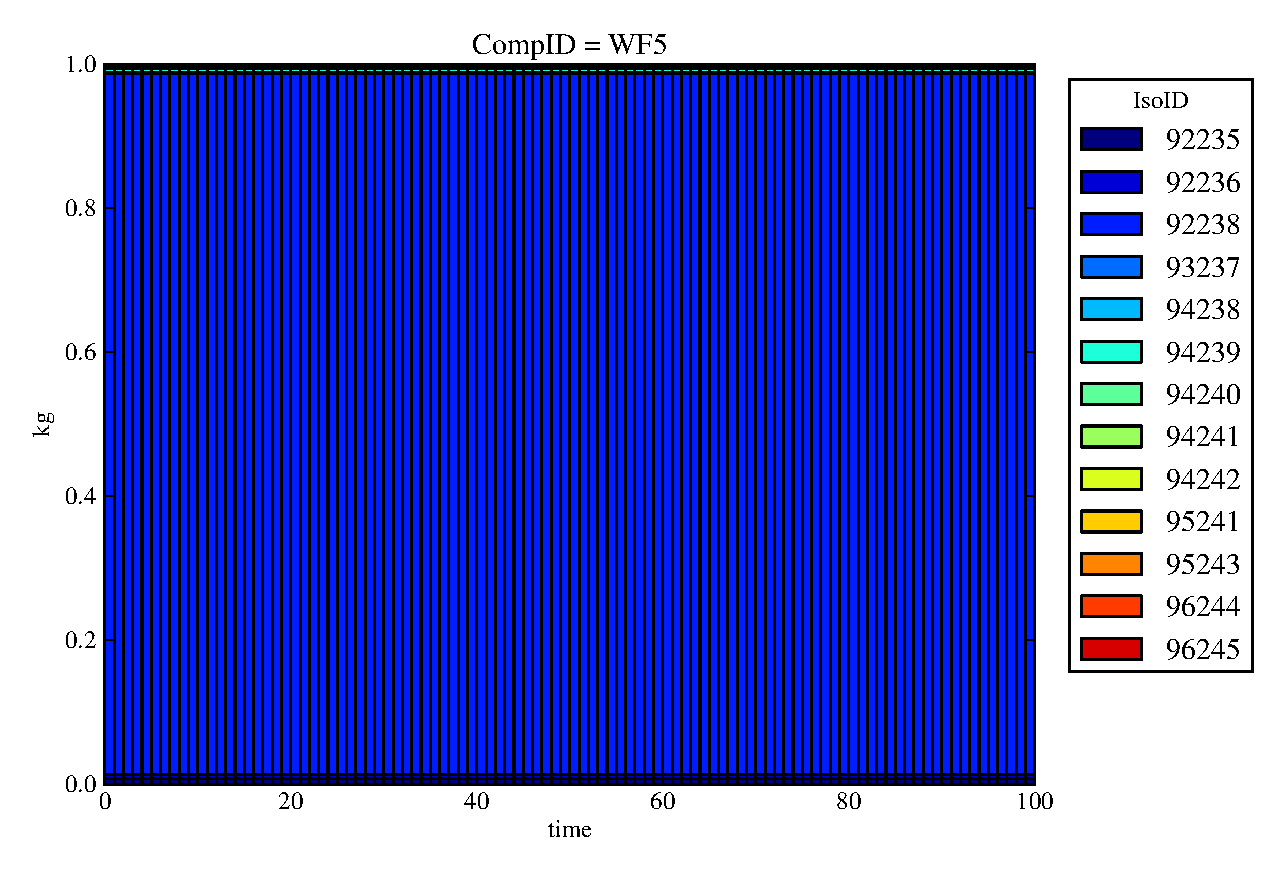
\includegraphics[width=\textwidth]{./chapters/demonstration/base/lpPFMII1.eps}
  \caption[Case LPPFMII Waste Form Contaminants.]{
    Waste Form 5 releases material. 
    }
  \label{fig:lpPFMIIwf5}
  \includegraphics[width=\textwidth]{./chapters/demonstration/base/lpPFMII3.eps}
  \caption[Case LPPFMII Buffer Contaminants]{
    The Buffer, component 7, never receives material.
    }
  \label{fig:lpPFMIIbuff}

\end{minipage}
\hspace{0.05\linewidth}
\begin{minipage}[b]{0.45\linewidth}
  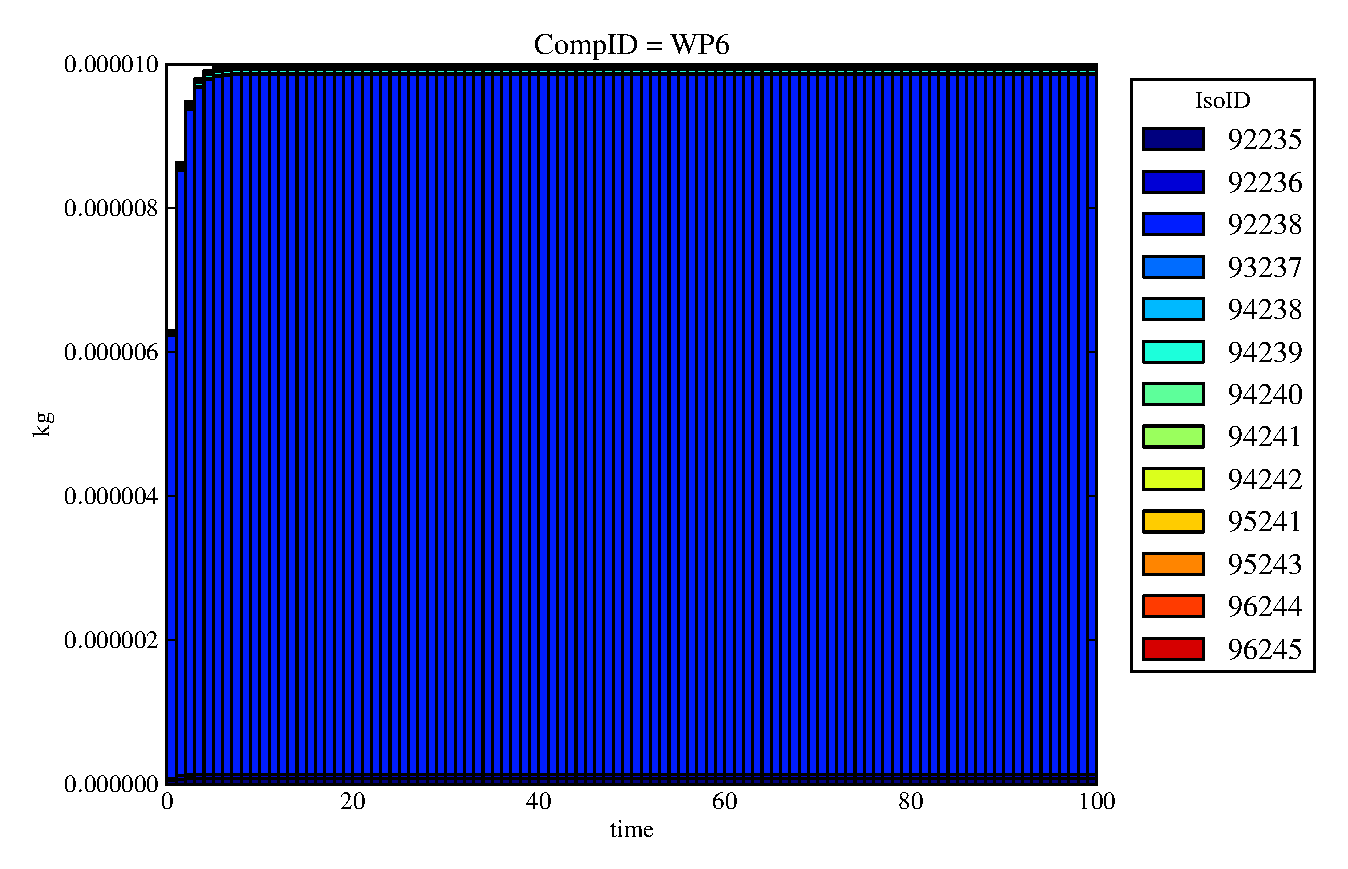
\includegraphics[width=\textwidth]{./chapters/demonstration/base/lpPFMII2.eps}
  \caption[Case LPPFMII Waste Package Contaminants.]{ 
    Waste Package 6 achieves total containment. 
    }
  \label{fig:lpPFMIIwp6}

  \includegraphics[width=\textwidth]{./chapters/demonstration/base/lpPFMII0.eps}
  \caption[Case LPPFMII Far Field Contaminants.]{ 
    The Far Field, component 4, never receives material.
    }
  \label{fig:lpEnd}
  \end{minipage}
\end{figure} 

In the second of these simulations, the Exponential Model (EM) was 
selected from among the three response functions. 

\begin{figure}[ht]
\centering
\includegraphics[width=0.6\textwidth]{./chapters/demonstration/base/lpEMII.eps}
\caption[$^{235}U$ residence. Lumped Parameter  Waste Package No Release.]{
For the Exponential Model case, LPEMII, in which total containment in the waste 
package is expected, $^{235}U$ travels through the waste form component ($\theta 
= 0.1$) before permanent residence in the waste package component ($\theta = 
0.1$) because the buffer component accepts no material ($\theta = 0.0$).  }
\label{fig:lpBegin}
\begin{minipage}[b]{0.45\linewidth}

  \includegraphics[width=\textwidth]{./chapters/demonstration/base/lpEMII1.eps}
  \caption[Case LPEMII Waste Form Contaminants.]{
    Waste Form 5 releases material. 
    }
  \label{fig:lpEMIIwf5}
  
  \includegraphics[width=\textwidth]{./chapters/demonstration/base/lpEMII3.eps}
  \caption[Case LPEMII Buffer Contaminants]{
    The Buffer, component 7, never receives material.
    }
  \label{fig:lpEMIIbuff}

\end{minipage}
\hspace{0.05\linewidth}
\begin{minipage}[b]{0.45\linewidth}
  \includegraphics[width=\textwidth]{./chapters/demonstration/base/lpEMII2.eps}
  \caption[Case LPEMII Waste Package Contaminants.]{ 
    Waste Package 6 achieves total containment. 
    }
  \label{fig:lpEMIIwp6}

  \includegraphics[width=\textwidth]{./chapters/demonstration/base/lpEMII0.eps}
  \caption[Case LPEMII Far Field Contaminants.]{ 
    The Far Field, component 4, never receives material.
    }
  \label{fig:lpEMIIff0}


  \end{minipage}
\end{figure}

In the second of these simulations, the Dispersion Model (DM) was 
selected from among the three response functions. 

\begin{figure}[ht]
\centering
\includegraphics[width=0.6\textwidth]{./chapters/demonstration/base/lpDMII.eps}
\caption[$^{235}U$ residence. Lumped Parameter  DM Waste Package No Release.]{
For the Dispersion Model case, LPEMII, in which total containment in the waste 
package is expected, $^{235}U$ travels through the waste form component ($\theta 
= 0.1$) before permanent residence in the waste package component ($\theta = 
0.1$) because the buffer component accepts no material ($\theta = 0.0$).  }
\label{fig:lpDMIIall}
\begin{minipage}[b]{0.45\linewidth}

  \includegraphics[width=\textwidth]{./chapters/demonstration/base/lpDMII1.eps}
  \caption[Case LPDMII Waste Form Contaminants.]{
    Waste Form 5 releases material. 
    }
  \label{fig:lpDMIIwf5}
  
  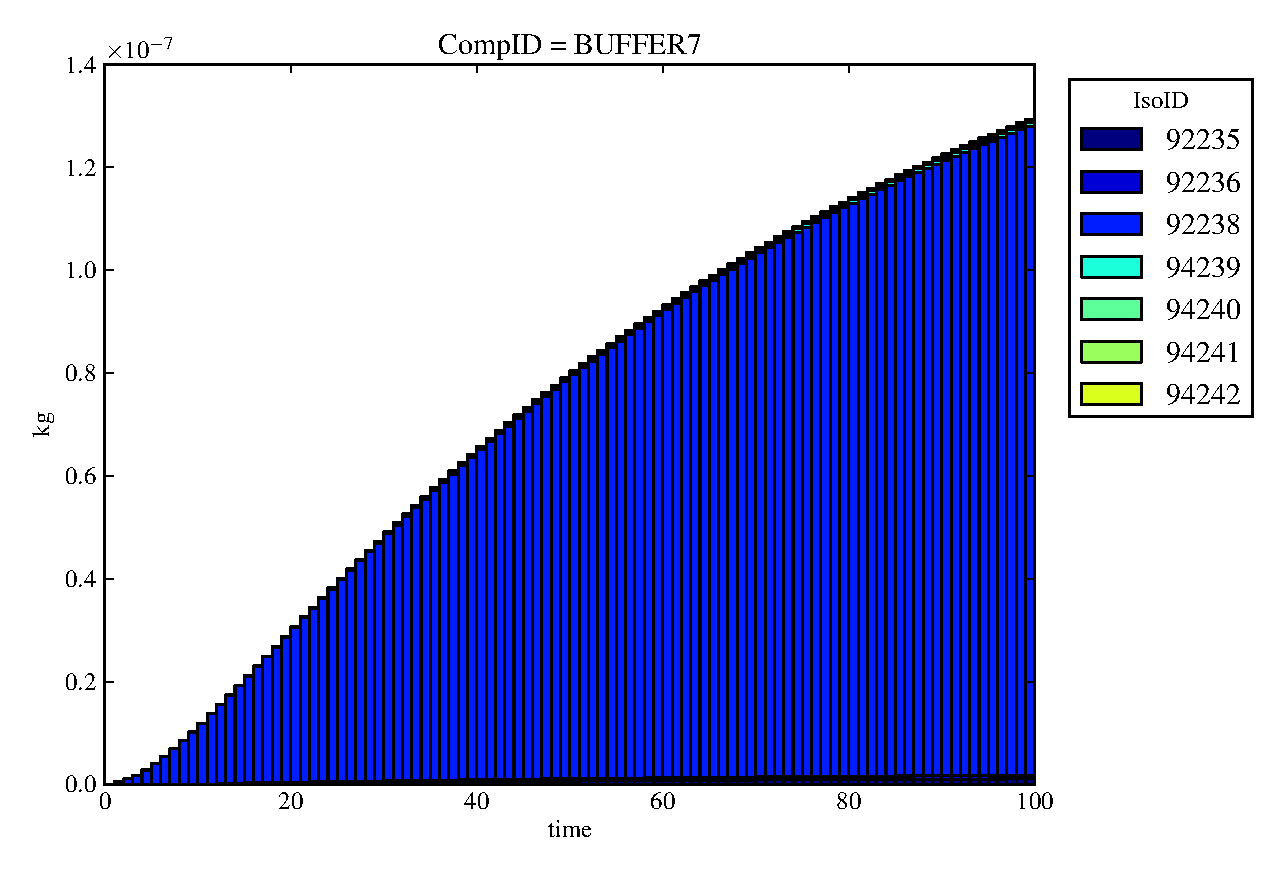
\includegraphics[width=\textwidth]{./chapters/demonstration/base/lpDMII3.eps}
  \caption[Case LPDMII Buffer Contaminants]{
    The Buffer, component 7, never receives material.
    }
  \label{fig:lpDMIIbuff}

\end{minipage}
\hspace{0.05\linewidth}
\begin{minipage}[b]{0.45\linewidth}
  \includegraphics[width=\textwidth]{./chapters/demonstration/base/lpDMII2.eps}
  \caption[Case LPDMII Waste Package Contaminants.]{ 
    Waste Package 6 achieves total containment. 
    }
  \label{fig:lpDMIIwp6}

  \includegraphics[width=\textwidth]{./chapters/demonstration/base/lpDMII0.eps}
  \caption[Case LPDMII Far Field Contaminants.]{ 
    The Far Field, component 4, never receives material.
    }
  \label{fig:lpDMIIff0}


  \end{minipage}
\end{figure}

\FloatBarrier
